\documentclass[11pt,a4paper]{article}

% Image mode: pdf.
% Image paths stay relative. In PDF mode, place same-basename PDF conversions
% of the chapter SVG files in the assets/ directory beside this source.

\usepackage{iftex}
\ifPDFTeX
  \PackageError{handout}{This template requires XeTeX or Tectonic}{Compile with xelatex or tectonic.}
\fi

\usepackage[a4paper,top=18mm,bottom=20mm,left=20mm,right=20mm,headsep=6mm]{geometry}
\usepackage{fontspec}
\usepackage{xeCJK}
\usepackage{amsmath}
\usepackage{unicode-math}

% Font settings are intentionally visible in the generated .tex file.
% These defaults target the macOS machine used for the released PDF.
% Change the family names when compiling on another system.
\setmainfont{Songti TC}
\setsansfont{Heiti TC}
\setmonofont{Menlo}
\setCJKmainfont{Songti TC}
\setCJKsansfont{Heiti TC}
\setCJKmonofont{Heiti TC}
\setmathfont{STIX Two Math}
\XeTeXlinebreaklocale "zh"
\XeTeXlinebreakskip=0pt plus 1pt

\usepackage{xcolor}
\definecolor{HandoutBlue}{HTML}{215A91}
\definecolor{HandoutBlueLight}{HTML}{EEF5FC}
\definecolor{HandoutGreen}{HTML}{39715A}
\definecolor{HandoutGreenLight}{HTML}{EFF8F3}
\definecolor{HandoutGold}{HTML}{8A641C}
\definecolor{HandoutGoldLight}{HTML}{FFF8E8}
\definecolor{HandoutInk}{HTML}{253142}
\definecolor{HandoutMuted}{HTML}{667085}

\usepackage{graphicx}
\makeatletter
% Pandoc 3 emits an accessibility `alt` key for raster/PDF images. Older
% graphicx releases do not know that key, so accept it without changing layout.
\@ifundefined{KV@Gin@alt}{\define@key{Gin}{alt}{}}{}
\newsavebox\pandoc@box
\newcommand*\pandocbounded[1]{%
  \sbox\pandoc@box{#1}%
  \Gscale@div\@tempa{\textheight}{\dimexpr\ht\pandoc@box+\dp\pandoc@box\relax}%
  \Gscale@div\@tempb{\linewidth}{\wd\pandoc@box}%
  \ifdim\@tempb\p@<\@tempa\p@\let\@tempa\@tempb\fi
  \ifdim\@tempa\p@<\p@\scalebox{\@tempa}{\usebox\pandoc@box}%
  \else\usebox{\pandoc@box}%
  \fi
}
\makeatother
\usepackage{float}
\floatplacement{figure}{H}
% Pandoc uses LTcaptype=none for uncaptioned longtables. The caption package
% expects that name to exist as a counter even though it is never displayed.
\newcounter{none}
\usepackage{caption}
\captionsetup[figure]{labelformat=empty,labelsep=none,font=small}

\usepackage{booktabs,longtable,array,calc}
\usepackage{etoolbox}
\makeatletter
\patchcmd\longtable{\par}{\if@noskipsec\mbox{}\fi\par}{}{}
\makeatother

\usepackage[most]{tcolorbox}
\tcbuselibrary{breakable,skins}
\newtcolorbox{HandoutLearningMap}{
  enhanced,breakable,colback=HandoutBlueLight,colframe=HandoutBlue,
  boxrule=0.8pt,arc=1.5mm,left=3mm,right=3mm,top=2mm,bottom=2mm,
  before skip=8pt,after skip=10pt
}
\newtcolorbox{HandoutWorkedExample}{
  enhanced,breakable,colback=HandoutGreenLight,colframe=HandoutGreen,
  boxrule=0.65pt,arc=1.5mm,left=3mm,right=3mm,top=2mm,bottom=2mm,
  before skip=8pt,after skip=10pt
}
\newtcolorbox{HandoutSelfCheck}{
  enhanced,breakable,colback=HandoutGoldLight,colframe=HandoutGold,
  boxrule=0.65pt,arc=1.5mm,left=3mm,right=3mm,top=2mm,bottom=2mm,
  before skip=8pt,after skip=10pt
}

\usepackage{titlesec}
\titleformat{\section}{\sffamily\bfseries\Large\color{HandoutBlue}}{}{0pt}{}
\titleformat{\subsection}{\sffamily\bfseries\large\color{HandoutInk}}{}{0pt}{}
\titleformat{\subsubsection}{\sffamily\bfseries\normalsize\color{HandoutInk}}{}{0pt}{}
\titlespacing*{\section}{0pt}{1.4em}{0.55em}
\titlespacing*{\subsection}{0pt}{1.15em}{0.45em}
\titlespacing*{\subsubsection}{0pt}{0.9em}{0.35em}
\setcounter{secnumdepth}{-\maxdimen}

\usepackage{hyperref}
\usepackage{bookmark}
\IfFileExists{xurl.sty}{\usepackage{xurl}}{}
\urlstyle{same}
\hypersetup{
  colorlinks=true,
  linkcolor=HandoutBlue,
  urlcolor=HandoutBlue,
  citecolor=HandoutBlue,
  pdftitle={數A3-2 指數與對數函數},
  pdfsubject={數學},
  pdfcreator={Pandoc with the HighSchooContent LaTeX template}
}

\setlength{\parindent}{0pt}
\setlength{\parskip}{0.55em plus 0.15em minus 0.1em}
\setlength{\emergencystretch}{3em}
\setlength{\LTpre}{0.5em}
\setlength{\LTpost}{0.5em}
\renewcommand{\arraystretch}{1.18}
\providecommand{\tightlist}{%
  \setlength{\itemsep}{0pt}\setlength{\parskip}{0pt}}
\pagestyle{plain}


\begin{document}

\begin{tcolorbox}[
  enhanced,colback=white,colframe=HandoutBlue,boxrule=1.1pt,arc=2mm,
  borderline west={3pt}{0pt}{HandoutBlue},left=5mm,right=4mm,top=4mm,bottom=4mm
]
{\sffamily\small\bfseries\color{HandoutBlue}學生講義}\par
{\sffamily\bfseries\LARGE\color{HandoutInk}數A3-2 指數與對數函數}\par
\vspace{0.35em}{\large 用倍率描述變化，再用對數倒推出需要幾步}\par
\vspace{0.45em}{\small\color{HandoutMuted}%
科目：數學
\quad 課程：普通高中數學A 第三冊
\quad 版本：學生版｜核心＋理解
\quad 校訂：2026-08-25
}\par
\vspace{0.25em}{\small\color{HandoutMuted}範圍：現行數學A主線}\par
\end{tcolorbox}


\begin{HandoutLearningMap}

\subsection{本章核心問題}\label{ux672cux7ae0ux6838ux5fc3ux554fux984c}

\begin{enumerate}
\def\labelenumi{\arabic{enumi}.}
\tightlist
\item
  \textbf{每一期都乘同一倍率，長期會怎麼變？}──指數函數描述按比例成長或衰退。
\item
  \textbf{想知道「要經過幾期」怎麼辦？}──對數把未知數從指數位置取回來。
\item
  \textbf{為什麼對數能把乘法變加法？}──因為它讀的是指數，而相乘時指數相加。
\item
  \textbf{這套語言實際用在哪裡？}──複利、衰減、演算法步數與分貝都在處理倍率。
\end{enumerate}

{藍色：現行核心}
{青綠：理解支援}
{紫色：延伸內容}

111--115 官方題本固定窗口中，5/5 份學測數學 A、5/5 份分科測驗數學甲至少有一題使用本章概念；這只描述已觀察試卷，不代表未來每年必考。

\end{HandoutLearningMap}

\section{0. 指數律與常用對數}\label{ux6307ux6578ux5f8bux8207ux5e38ux7528ux5c0dux6578}

本章會反覆用到指數律。對 \(a>0\)、實數 \(m,n\)：

\[
a^m a^n=a^{m+n},\qquad
\frac{a^m}{a^n}=a^{m-n},\qquad
(a^m)^n=a^{mn},\qquad
a^{-n}=\frac1{a^n}.
\]

高一也已把常用對數定義為

\[
\boxed{\log N=y\iff 10^y=N},\qquad N>0.
\]

例如 \(\log1000=3\)，因為 \(10^3=1000\)。

\begin{HandoutSelfCheck}

\subsection{練習｜指數律與常用對數}\label{ux7df4ux7fd2ux6307ux6578ux5f8bux8207ux5e38ux7528ux5c0dux6578}

將 \(8^{x-1}\) 化為底數 \(2\)；並求 \(\log0.01\)。

\textbf{答案：}\(8^{x-1}=(2^3)^{x-1}=2^{3x-3}\)；\(0.01=10^{-2}\)，所以 \(\log0.01=-2\)。

\end{HandoutSelfCheck}

\section{1. 指數函數：重複的倍率累積成曲線}\label{ux6307ux6578ux51fdux6578ux91cdux8907ux7684ux500dux7387ux7d2fux7a4dux6210ux66f2ux7dda}

\subsection{\texorpdfstring{1.1 為什麼會出現 \(a^x\)？}{1.1 為什麼會出現 a\^{}x？}}\label{ux70baux4ec0ux9ebcux6703ux51faux73fe-ax}

固定增加與固定倍率是兩種不同的變化：

{\def\LTcaptype{none} % do not increment counter
\begin{longtable}[]{@{}llll@{}}
\toprule\noalign{}
規則 & 每期更新 & \(n\) 期後 & 典型模型 \\
\midrule\noalign{}
\endhead
\bottomrule\noalign{}
\endlastfoot
固定增加 \(d\) & \(Q_{n+1}=Q_n+d\) & \(Q_n=Q_0+nd\) & 線性 \\
固定乘倍率 \(a\) & \(Q_{n+1}=aQ_n\) & \(Q_n=Q_0a^n\) & 指數 \\
\end{longtable}
}

從 \(Q_0\) 出發，做一次得到 \(Q_0a\)，做兩次得到 \(Q_0a^2\)；做 \(n\) 次自然得到 \(Q_0a^n\)。指數精確表示\textbf{同一倍率重複累積}。

\subsection{指數模型如何描述按比例變化？}\label{ux6307ux6578ux6a21ux578bux5982ux4f55ux63cfux8ff0ux6309ux6bd4ux4f8bux8b8aux5316}

\textbf{適用情況。} 利息、衰減或早期族群變化常依「目前有多少」決定下一期改變多少；固定比例變化對應指數模型，固定加量對應線性模型。

\textbf{次方的來源。} 每一期都把目前量乘同一倍率；倍率重複 \(n\) 次就是 \(a^n\)。

\textbf{從離散期數延伸到連續時間。} 連續時間包含任意實數時刻。把 \(Q=Q_0a^x\) 視為函數，便能估計半期、任意時刻，並用圖形比較成長與衰退。

\textbf{應用與限制。} 複利帳戶用 \(P(1+r)^n\)；固定比例折舊或衰減用 \(Q_0a^t\)。模型適用於倍率可視為固定的研究區間，外推範圍也受此前提限制。

\subsection{1.2 定義、圖形與底數}\label{ux5b9aux7fa9ux5716ux5f62ux8207ux5e95ux6578}

取 \(a>0\) 且 \(a\ne1\)，

\[
\boxed{f(x)=a^x}
\]

稱為以 \(a\) 為底的指數函數。它的定義域為 \(\mathbb R\)，值域為 \((0,\infty)\)。

排除 \(a\le0\)，是因為要讓每個實數 \(x\) 都有實數函數值；排除 \(a=1\)，是因為 \(1^x\equiv1\) 只是常數函數。

{\def\LTcaptype{none} % do not increment counter
\begin{longtable}[]{@{}lll@{}}
\toprule\noalign{}
條件 & \(a>1\) & \(0<a<1\) \\
\midrule\noalign{}
\endhead
\bottomrule\noalign{}
\endlastfoot
單調性 & 嚴格遞增 & 嚴格遞減 \\
共同定點 & \((0,1)\) & \((0,1)\) \\
水平漸近線 & \(y=0\) & \(y=0\) \\
\(x\) 增大時 & 函數值增大 & 函數值減小 \\
\end{longtable}
}

兩種圖形都在 \(x\) 軸上方，也都凹口向上。現行教材以圖形觀察凹口向上：兩點間的弦落在曲線上方；微積分證明留待後續課程。

而且

\[
\left(\frac1a\right)^x=a^{-x},
\]

所以 \(y=a^x\) 與 \(y=(1/a)^x\) 對 \(y\) 軸對稱。

同一個 \(x\) 對不同底數的影響，可由數值表直接比較：

{\def\LTcaptype{none} % do not increment counter
\begin{longtable}[]{@{}rrrr@{}}
\toprule\noalign{}
\(x\) & \(2^x\) & \(4^x\) & \((1/2)^x\) \\
\midrule\noalign{}
\endhead
\bottomrule\noalign{}
\endlastfoot
\(-2\) & \(1/4\) & \(1/16\) & \(4\) \\
\(-1\) & \(1/2\) & \(1/4\) & \(2\) \\
\(0\) & \(1\) & \(1\) & \(1\) \\
\(1\) & \(2\) & \(4\) & \(1/2\) \\
\(2\) & \(4\) & \(16\) & \(1/4\) \\
\end{longtable}
}

當 \(x>0\) 時，較大的底數成長較快；當 \(x<0\) 時，負指數會取倒數，次序隨之反轉。三條曲線都通過 \((0,1)\)，比較底數前要同時注意 \(x\) 的正負。

\subsection{1.3 圖形變換怎麼讀}\label{ux5716ux5f62ux8b8aux63dbux600eux9ebcux8b80}

對底數 \(a>0\)、\(a\ne1\)，且非退化情形 \(A\ne0\)、\(B\ne0\) 的

\[
y=Aa^{B(x-h)}+D,
\]

先看 \(a^{B(x-h)}>0\)，再依序處理：

\begin{itemize}
\tightlist
\item
  \(h\)：水平位移；
\item
  \(B\)：水平方向的伸縮與左右方向；若只問基本課程常見型，先把括號整理成 \(B(x-h)\)；
\item
  \(A\)：鉛直伸縮，\(A<0\) 時再上下翻轉；
\item
  \(D\)：鉛直平移；原本的漸近線 \(y=0\) 變成 \(y=D\)。
\end{itemize}

若 \(A=0\) 或 \(B=0\)，函數退化為常數函數，需改按常數函數判讀；先檢查參數條件，再套用圖形語言。

\begin{HandoutWorkedExample}

\subsection{完整示範｜由參數判讀指數圖形}\label{ux5b8cux6574ux793aux7bc4ux7531ux53c3ux6578ux5224ux8b80ux6307ux6578ux5716ux5f62}

分析

\[
f(x)=2\left(\frac12\right)^{x-3}-1.
\]

底數 \(1/2<1\)，基本圖形遞減；乘正數 \(2\) 不改方向，右移 \(3\)、下移 \(1\)。因此：

\begin{itemize}
\tightlist
\item
  定義域 \(\mathbb R\)；
\item
  值域 \((-1,\infty)\)；
\item
  水平漸近線 \(y=-1\)；
\item
  \(f(3)=2(1)-1=1\)，圖形通過 \((3,1)\)。
\end{itemize}

代回 \(x=3\) 可檢查位移方向。

\end{HandoutWorkedExample}

\subsection{常見錯誤｜把「越來越接近 0」說成「等於 0」}\label{ux5e38ux898bux932fux8aa4ux628aux8d8aux4f86ux8d8aux63a5ux8fd1-0ux8aaaux6210ux7b49ux65bc-0}

\(a^x\) 可以無限接近 \(0\)，但永遠為正；因此基本指數函數沒有 \(x\) 截距。平移後的 \(Aa^{B(x-h)}+D\) 則需另行解方程式判斷截距。

\begin{HandoutSelfCheck}

\subsection{練習｜指數圖形}\label{ux7df4ux7fd2ux6307ux6578ux5716ux5f62}

\(g(x)=3^{x+2}+4\) 的水平漸近線、值域與 \(g(-2)\) 各為何？

\textbf{答案：}水平漸近線 \(y=4\)；值域 \((4,\infty)\)；\(g(-2)=5\)。

\end{HandoutSelfCheck}

\begin{HandoutWorkedExample}

\subsection{完整示範｜由漸近線與已知點決定函數}\label{ux5b8cux6574ux793aux7bc4ux7531ux6f38ux8fd1ux7ddaux8207ux5df2ux77e5ux9edeux6c7aux5b9aux51fdux6578}

函數

\[
f(x)=A\cdot2^x+D
\]

的水平漸近線為 \(y=-2\)，且通過 \((0,1)\)。求 \(f(x)\)，並判斷單調性和值域。

水平漸近線直接給出 \(D=-2\)。再代入 \((0,1)\)：

\[
1=A\cdot2^0-2=A-2,
\]

所以 \(A=3\)，

\[
\boxed{f(x)=3\cdot2^x-2}.
\]

底數 \(2>1\) 且 \(A>0\)，因此函數嚴格遞增。又 \(3\cdot2^x>0\)，故值域為

\[
\boxed{(-2,\infty)}.
\]

把 \(x=0\) 代回得 \(1\)，與已知點一致。

\end{HandoutWorkedExample}

\subsection{1.4 指數方程式與不等式}\label{ux6307ux6578ux65b9ux7a0bux5f0fux8207ux4e0dux7b49ux5f0f}

解題前先判斷是哪一種結構：

\begin{enumerate}
\def\labelenumi{\arabic{enumi}.}
\tightlist
\item
  \textbf{化同底}：\(a^{u(x)}=a^{v(x)}\Rightarrow u(x)=v(x)\)。
\item
  \textbf{換元}：若同時出現 \(a^{2x}\)、\(a^x\)，令 \(t=a^x>0\)。
\item
  \textbf{異底方程}：化不成同底時，待第 2 節定義對數、換底與自然對數後，再把未知指數移到一般代數位置。
\end{enumerate}

\begin{HandoutWorkedExample}

\subsection{\texorpdfstring{完整示範｜換元條件 \(t>0\)}{完整示範｜換元條件 t\textgreater0}}\label{ux5b8cux6574ux793aux7bc4ux63dbux5143ux689dux4ef6-t0}

解

\[
4^x-5\cdot2^x+4=0.
\]

令 \(t=2^x>0\)，則 \(4^x=t^2\)：

\[
t^2-5t+4=(t-1)(t-4)=0.
\]

所以 \(t=1\) 或 \(4\)，回代得

\[
2^x=1\Rightarrow x=0,\qquad
2^x=4\Rightarrow x=2.
\]

故 \(\boxed{x=0,2}\)。

\end{HandoutWorkedExample}

不等式的方向由函數單調性決定：

對 \(a>0\)、\(a\ne1\)，

\[
a>1:\quad a^u>a^v\iff u>v,
\]

\[
0<a<1:\quad a^u>a^v\iff u<v.
\]

底數小於 \(1\) 時不等號反向，源於 \(y=a^x\) 為遞減函數。

\begin{HandoutSelfCheck}

\subsection{練習｜指數不等式}\label{ux7df4ux7fd2ux6307ux6578ux4e0dux7b49ux5f0f}

解 \((1/3)^{2x-1}\ge27\)。

\textbf{答案：}\(27=(1/3)^{-3}\)。底數小於 \(1\)，所以 \(2x-1\le-3\)，得 \(\boxed{x\le-1}\)。

\end{HandoutSelfCheck}

\begin{HandoutWorkedExample}

\subsection{完整示範｜換元後用平方完成求極值}\label{ux5b8cux6574ux793aux7bc4ux63dbux5143ux5f8cux7528ux5e73ux65b9ux5b8cux6210ux6c42ux6975ux503c}

求

\[
f(x)=4^x-6\cdot2^x+5
\]

的最小值及取得位置。

令 \(t=2^x\)。因 \(2^x>0\)，所以 \(t>0\)，且 \(4^x=t^2\)：

\[
f=t^2-6t+5=(t-3)^2-4.
\]

\(t=3\) 符合 \(t>0\)，因此

\[
\boxed{f_{\min}=-4}.
\]

取得位置是滿足 \(\boxed{2^x=3}\) 的唯一實數；第 2 節定義對數後，可把這個位置寫成對數形式。

平方項永遠非負，且等號可由實數 \(x\) 取得，所以此下界就是最小值。

\end{HandoutWorkedExample}

\begin{HandoutSelfCheck}

\subsection{節末練習｜指數圖形、方程式與極值}\label{ux7bc0ux672bux7df4ux7fd2ux6307ux6578ux5716ux5f62ux65b9ux7a0bux5f0fux8207ux6975ux503c}

\begin{enumerate}
\def\labelenumi{\arabic{enumi}.}
\tightlist
\item
  比較 \(3^{-2}\)、\(5^{-2}\) 的大小，並用負指數說明理由。
\item
  求 \(y=-2\cdot3^{x+1}+4\) 的漸近線、值域與單調性。
\item
  解 \(8^{x-1}=4^{2x+1}\)。
\item
  解 \(5^{2x}-26\cdot5^x+25=0\)。
\item
  解 \((1/2)^{x-3}\le8\)。
\item
  求 \(9^x-8\cdot3^x+7\) 的最小值與取得位置。
\end{enumerate}

\textbf{答案：}

\begin{enumerate}
\def\labelenumi{\arabic{enumi}.}
\tightlist
\item
  \(3^{-2}=1/9>1/25=5^{-2}\)；底數較大，平方後倒數較小。
\item
  漸近線 \(y=4\)；值域 \((-\infty,4)\)；嚴格遞減。
\item
  \(2^{3x-3}=2^{4x+2}\)，所以 \(x=-5\)。
\item
  令 \(t=5^x>0\)，得 \((t-1)(t-25)=0\)，所以 \(x=0,2\)。
\item
  \(8=(1/2)^{-3}\)；底數小於 \(1\)，故 \(x-3\ge-3\)，即 \(x\ge0\)。
\item
  令 \(t=3^x>0\)，則 \(t^2-8t+7=(t-4)^2-9\)；最小值 \(-9\)，在滿足 \(3^x=4\) 的唯一實數 \(x\) 取得。
\end{enumerate}

\end{HandoutSelfCheck}

\section{2. 對數：把「冪值」倒查成「指數」}\label{ux5c0dux6578ux628aux51aaux503cux5012ux67e5ux6210ux6307ux6578}

\subsection{2.1 一般對數與反函數}\label{ux4e00ux822cux5c0dux6578ux8207ux53cdux51fdux6578}

對 \(a>0\)、\(a\ne1\)、\(x>0\)，

\[
\boxed{y=\log_a x\iff a^y=x}.
\]

\(y=\log_a x\) 稱為以 \(a\) 為底的對數函數；定義域是 \((0,\infty)\)，值域是 \(\mathbb R\)。

指數函數輸入「指數」並輸出「冪值」；對數函數輸入「冪值」並輸出「指數」。所以

\[
\log_a(a^x)=x,\qquad a^{\log_a x}=x\quad(x>0).
\]

圖 1 取 \(a=2\)。指數圖上的 \((p,q)\) 對應對數圖上的 \((q,p)\)；例如
\((0,1)\leftrightarrow(1,0)\)、\((1,2)\leftrightarrow(2,1)\)。虛線 \(y=x\)
是鏡射軸，兩條函數曲線分居其兩側，沒有交在鏡射軸上。

\begin{figure}
\centering
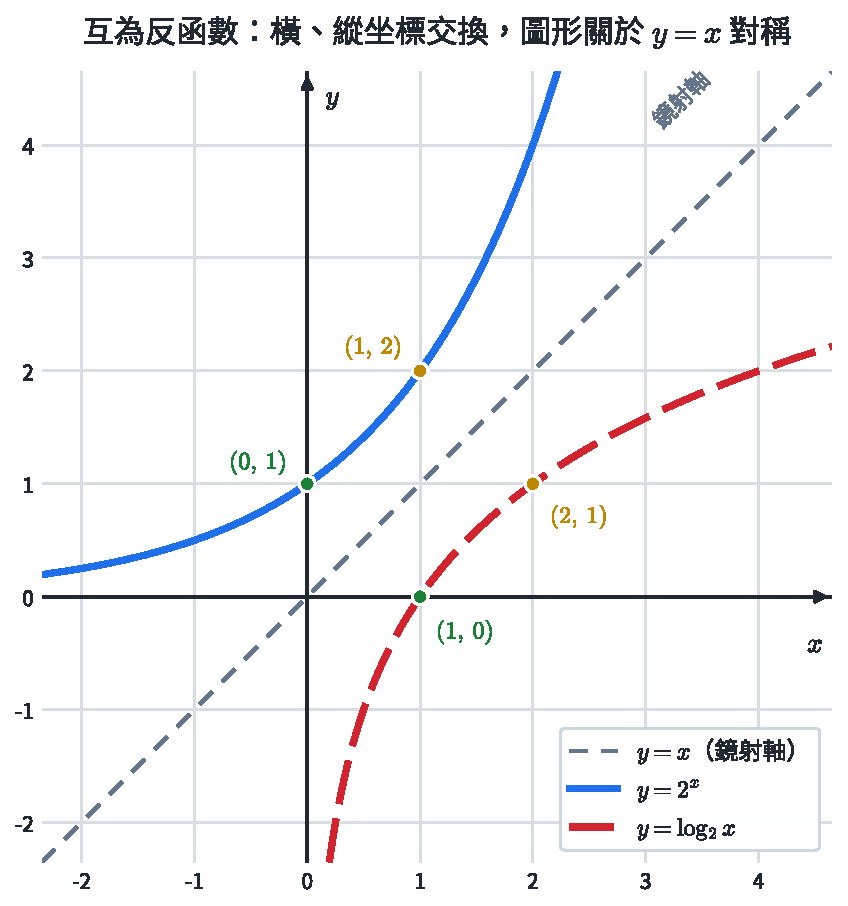
\includegraphics[width=0.96\linewidth,height=\textheight,keepaspectratio,alt={圖 1｜y=2\^{}x 與 y=\textbackslash log\_2x 關於 y=x 對稱；同色點的橫、縱坐標互換，虛線只表示鏡射軸。}]{assets/數A3-2-指數對數互逆.pdf}
\caption{圖 1｜\(y=2^x\) 與 \(y=\log_2x\) 關於 \(y=x\) 對稱；同色點的橫、縱坐標互換，虛線只表示鏡射軸。}
\end{figure}

\subsection{對數如何求出未知的指數？}\label{ux5c0dux6578ux5982ux4f55ux6c42ux51faux672aux77e5ux7684ux6307ux6578}

\textbf{問題結構。} \(Q=Q_0a^t\) 可由時間算數量；要求「到達目標需幾期」時，未知數位於指數位置。

\textbf{反函數解出指數。} \(\log_a\) 是 \(a^x\) 的反函數：\(a^t=M\) 等價於 \(t=\log_a M\)。

\textbf{圖形對稱。} 指數圖上的 \((p,q)\) 表示 \(a^p=q\)；倒過來就是 \(\log_a q=p\)，所以對數圖上有 \((q,p)\)。交換橫、縱坐標正是對 \(y=x\) 鏡射。

\textbf{應用。} 求複利多久達標、某量要經幾次減半、二分搜尋最多要切幾次，都是「已知結果，倒查步數」。

對數函數的性質也由反函數關係直接得到：

{\def\LTcaptype{none} % do not increment counter
\begin{longtable}[]{@{}lll@{}}
\toprule\noalign{}
條件 & \(a>1\) & \(0<a<1\) \\
\midrule\noalign{}
\endhead
\bottomrule\noalign{}
\endlastfoot
單調性 & 嚴格遞增 & 嚴格遞減 \\
共同定點 & \((1,0)\) & \((1,0)\) \\
鉛直漸近線 & \(x=0\) & \(x=0\) \\
\end{longtable}
}

\subsection{對數的定義域}\label{ux5c0dux6578ux7684ux5b9aux7fa9ux57df}

對數的真數必須大於 \(0\)。例如 \(\log_2(x-3)\) 的定義域是 \(x>3\)；解方程或不等式時，必須先列真數條件並在最後檢查。

\begin{HandoutSelfCheck}

\subsection{練習｜反函數}\label{ux7df4ux7fd2ux53cdux51fdux6578}

指數圖上的點 \((-2,1/9)\) 對應到哪一個以 \(3\) 為底的對數敘述？

\textbf{答案：}\(3^{-2}=1/9\)，因此 \(\log_3(1/9)=-2\)；對數圖上對應點為 \((1/9,-2)\)。

\end{HandoutSelfCheck}

\subsection{2.2 對數律：乘法為什麼變加法}\label{ux5c0dux6578ux5f8bux4e58ux6cd5ux70baux4ec0ux9ebcux8b8aux52a0ux6cd5}

若 \(M=a^u\)、\(N=a^v\)，則 \(MN=a^{u+v}\)。對數讀出指數，所以乘法自然變成加法：

對 \(a>0\)、\(a\ne1\)，且 \(M,N>0\)，

\[
\boxed{\log_a(MN)=\log_aM+\log_aN},
\]

\[
\boxed{\log_a\frac MN=\log_aM-\log_aN},
\]

\[
\boxed{\log_a(M^r)=r\log_aM}.
\]

這三式是指數律的反向翻譯，不適用於真數的加減：

\[
\log_a(M+N)\ne\log_aM+\log_aN.
\]

\begin{HandoutWorkedExample}

\subsection{完整示範｜先看結構再拆}\label{ux5b8cux6574ux793aux7bc4ux5148ux770bux7d50ux69cbux518dux62c6}

已知 \(\log2\approx0.3010\)、\(\log3\approx0.4771\)，估算 \(\log7.2\)。

因為 \(7.2=72/10=2^3\cdot3^2/10\)，

\[
\begin{aligned}
\log7.2
&=3\log2+2\log3-1\\
&\approx3(0.3010)+2(0.4771)-1\\
&=\boxed{0.8572}.
\end{aligned}
\]

答案在 \(0\) 與 \(1\) 之間也合理，因為 \(1<7.2<10\)。

\end{HandoutWorkedExample}

\subsection{2.3 換底公式}\label{ux63dbux5e95ux516cux5f0f}

換底公式可把任意底的對數改寫成計算機提供的常用對數。設 \(t=\log_a b\)，則 \(a^t=b\)。兩邊取常用對數：

\[
t\log a=\log b.
\]

所以

\[
\boxed{\log_a b=\frac{\log b}{\log a}}.
\]

更一般地，只要 \(c>0\)、\(c\ne1\)，

\[
\log_a b=\frac{\log_c b}{\log_c a}.
\]

分子是真數 \(b\) 的對數，分母是原底數 \(a\) 的對數。由此也得到

\[
\log_a b=\frac1{\log_b a}.
\]

\subsection{換底為何保持對數值？}\label{ux63dbux5e95ux70baux4f55ux4fddux6301ux5c0dux6578ux503c}

\(\log_a b\) 是滿足 \(a^t=b\) 的那個固定數 \(t\)；換底只是改用另一種刻度表示。分子與分母一起換，比例不變。實務上可換成計算機提供的常用對數；下一節定義自然對數後，也可用 \(\ln\) 計算。

\subsection{\texorpdfstring{2.4 自然對數 \(e\) 與 \(\ln\)}{2.4 自然對數 e 與 \textbackslash ln}}\label{ux81eaux7136ux5c0dux6578-e-ux8207-ln}

\[
\boxed{e\approx2.71828},
\qquad
\boxed{\ln x=\log_e x}\quad(x>0).
\]

\(e\) 是合法的對數底數，\(\ln\) 是以 \(e\) 為底的對數。因此一般對數的定義、對數律與換底公式都可直接使用；本章使用 \(e\)、\(\ln\) 的數值與記號，極限定義、導數及連續成長理論留到微積分。

\subsection{\texorpdfstring{複利切分如何產生 \(e\)？}{複利切分如何產生 e？}}\label{ux8907ux5229ux5207ux5206ux5982ux4f55ux7522ux751f-e}

若本金為 \(1\)，一年的總利率為 \(100\%\)，平均切成 \(n\) 次複利，一年後的本利和為

\[
\left(1+\frac1n\right)^n.
\]

{\def\LTcaptype{none} % do not increment counter
\begin{longtable}[]{@{}rr@{}}
\toprule\noalign{}
一年計息次數 \(n\) & \(\left(1+\dfrac1n\right)^n\) \\
\midrule\noalign{}
\endhead
\bottomrule\noalign{}
\endlastfoot
\(1\) & \(2.0000\) \\
\(2\) & \(2.2500\) \\
\(4\) & \(2.4414\) \\
\(12\) & \(2.6130\) \\
\(365\) & \(2.7146\) \\
\end{longtable}
}

切分愈細時，數值趨近 \(e\approx2.71828\)。表格提供 \(e\) 的來源動機；證明極限存在需要後續的極限工具。

\begin{HandoutWorkedExample}

\subsection{完整示範｜異底指數方程式用自然對數解}\label{ux5b8cux6574ux793aux7bc4ux7570ux5e95ux6307ux6578ux65b9ux7a0bux5f0fux7528ux81eaux7136ux5c0dux6578ux89e3}

解

\[
3^{2x-1}=5^{x+1}.
\]

兩邊皆為正，可取自然對數：

\[
(2x-1)\ln3=(x+1)\ln5.
\]

把含 \(x\) 的項放在同一邊：

\[
x(2\ln3-\ln5)=\ln3+\ln5.
\]

因 \(2\ln3-\ln5=\ln(9/5)>0\)，所以

\[
\boxed{x=\frac{\ln3+\ln5}{2\ln3-\ln5}}
\approx4.61.
\]

近似代回時，兩邊的自然對數都約為 \(7.02\)，小數差異來自截位。

\end{HandoutWorkedExample}

\begin{HandoutSelfCheck}

\subsection{題組｜2-2 對數、對數律與換底}\label{ux984cux7d442-2-ux5c0dux6578ux5c0dux6578ux5f8bux8207ux63dbux5e95}

\begin{enumerate}
\def\labelenumi{\arabic{enumi}.}
\tightlist
\item
  求 \(\log_2(1/8)\)、\(\log_{1/3}27\) 與 \(4^{\log_4 7}\)。
\item
  已知 \(\log2=p\)、\(\log3=q\)，以 \(p,q\) 表示 \(\log75\)。
\item
  化簡 \(\log_a(9x^2)-2\log_a(3x)\)，其中 \(a>0\)、\(a\ne1\)、\(x>0\)。
\item
  化簡 \(\log_2 3\cdot\log_3 8\)。
\item
  解 \(\log_2(x+3)-\log_2(x-1)=2\)。
\end{enumerate}

\textbf{答案：}

\begin{enumerate}
\def\labelenumi{\arabic{enumi}.}
\tightlist
\item
  \(-3\)、\(-3\)、\(7\)。
\item
  \(75=3\cdot5^2\) 且 \(\log5=1-p\)，所以 \(\log75=q+2(1-p)=2-2p+q\)。
\item
  \(\log_a(9x^2)-\log_a(9x^2)=0\)；條件 \(x>0\) 使原式各真數有意義。
\item
  \(\log_3 8=\log_2 8/\log_2 3\)，所以乘積為 \(\log_2 8=3\)。
\item
  先有 \(x>1\)；\(\log_2\dfrac{x+3}{x-1}=2\)，故 \((x+3)/(x-1)=4\)，得 \(x=7/3\)。
\end{enumerate}

\end{HandoutSelfCheck}

\subsection{2.5 對數圖形的位移、底數與凹向}\label{ux5c0dux6578ux5716ux5f62ux7684ux4f4dux79fbux5e95ux6578ux8207ux51f9ux5411}

基本對數函數除單調性外，還可由圖形比較彎曲方向：

{\def\LTcaptype{none} % do not increment counter
\begin{longtable}[]{@{}
  >{\raggedright\arraybackslash}p{(\linewidth - 4\tabcolsep) * \real{0.3333}}
  >{\raggedright\arraybackslash}p{(\linewidth - 4\tabcolsep) * \real{0.3333}}
  >{\raggedright\arraybackslash}p{(\linewidth - 4\tabcolsep) * \real{0.3333}}@{}}
\toprule\noalign{}
\begin{minipage}[b]{\linewidth}\raggedright
條件
\end{minipage} & \begin{minipage}[b]{\linewidth}\raggedright
\(a>1\)
\end{minipage} & \begin{minipage}[b]{\linewidth}\raggedright
\(0<a<1\)
\end{minipage} \\
\midrule\noalign{}
\endhead
\bottomrule\noalign{}
\endlastfoot
單調性 & 嚴格遞增 & 嚴格遞減 \\
凹向 & 凹口向下；兩點間的弦落在曲線下方 & 凹口向上；兩點間的弦落在曲線上方 \\
\end{longtable}
}

對

\[
y=A\log_a(B(x-h))+D,
\]

先由真數條件 \(B(x-h)>0\) 決定定義域；使真數趨近 \(0^+\) 的直線是鉛直漸近線。\(D\) 控制鉛直平移，\(A\) 的正負會改變單調方向與凹向。對數圖形的漸近線是鉛直的，因為限制發生在輸入端。

若 \(1<a<b\)，換成已定義的常用對數：

\[
\log_a x=\frac{\log x}{\log a},
\qquad
\log_b x=\frac{\log x}{\log b},
\qquad
0<\log a<\log b.
\]

\begin{itemize}
\tightlist
\item
  \(x>1\) 時 \(\log x>0\)，所以 \(\log_a x>\log_b x\)；
\item
  \(0<x<1\) 時 \(\log x<0\)，除以較小正數會得到更小的負數，所以 \(\log_a x<\log_b x\)；
\item
  \(x=1\) 時兩者都為 \(0\)。
\end{itemize}

\begin{HandoutWorkedExample}

\subsection{完整示範｜由真數條件判讀平移後的對數圖}\label{ux5b8cux6574ux793aux7bc4ux7531ux771fux6578ux689dux4ef6ux5224ux8b80ux5e73ux79fbux5f8cux7684ux5c0dux6578ux5716}

分析

\[
g(x)=\log_2(x-3)+1.
\]

真數條件給

\[
x-3>0\Longrightarrow x>3,
\]

所以定義域是 \((3,\infty)\)，鉛直漸近線是 \(x=3\)。底數 \(2>1\)，圖形嚴格遞增且凹口向下；值域仍是 \(\mathbb R\)。

\(x\) 截距由 \(g(x)=0\) 求得：

\[
\log_2(x-3)=-1
\Longrightarrow x-3=\frac12
\Longrightarrow
\boxed{x=\frac72}.
\]

另外 \(g(4)=1\)，所以圖形通過 \((4,1)\)。這兩個點與漸近線足以校準草圖的位置。

\end{HandoutWorkedExample}

\subsection{2.6 對數方程式與不等式}\label{ux5c0dux6578ux65b9ux7a0bux5f0fux8207ux4e0dux7b49ux5f0f}

解對數方程式時：

\begin{enumerate}
\def\labelenumi{\arabic{enumi}.}
\tightlist
\item
  先列每個真數 \(>0\)；
\item
  用對數律合併；
\item
  由一對一性去掉同底對數；
\item
  最後檢查真數條件。
\end{enumerate}

\begin{HandoutWorkedExample}

\subsection{完整示範｜回代檢查對數定義域}\label{ux5b8cux6574ux793aux7bc4ux56deux4ee3ux6aa2ux67e5ux5c0dux6578ux5b9aux7fa9ux57df}

解

\[
\log_2(x-1)+\log_2(x-3)=3.
\]

先決條件為 \(x>3\)。合併後：

\[
\log_2[(x-1)(x-3)]=3
\]

\[
(x-1)(x-3)=8
\]

\[
x^2-4x-5=0
\Rightarrow (x-5)(x+1)=0.
\]

代數上得到 \(x=5,-1\)，但只有 \(x=5\) 滿足 \(x>3\)，所以

\[
\boxed{x=5}.
\]

\end{HandoutWorkedExample}

對數不等式與指數不等式同理：

在 \(M,N>0\) 的前提下，

\[
a>1:\quad \log_aM>\log_aN\iff M>N,
\]

\[
0<a<1:\quad \log_aM>\log_aN\iff M<N.
\]

\begin{HandoutSelfCheck}

\subsection{練習｜對數不等式}\label{ux7df4ux7fd2ux5c0dux6578ux4e0dux7b49ux5f0f}

解 \(\log_{1/2}(x+1)>-2\)。

\textbf{答案：}先有 \(x>-1\)。因底數小於 \(1\)，比較真數時反向：

\[
x+1<(1/2)^{-2}=4.
\]

故 \(\boxed{-1<x<3}\)。

\end{HandoutSelfCheck}

\begin{HandoutWorkedExample}

\subsection{完整示範｜不同底數先換成同一刻度}\label{ux5b8cux6574ux793aux7bc4ux4e0dux540cux5e95ux6578ux5148ux63dbux6210ux540cux4e00ux523bux5ea6}

解

\[
\log_2x+\log_4x=6.
\]

先有 \(x>0\)。由換底公式，

\[
\log_4x=\frac{\log_2x}{\log_24}=\frac12\log_2x.
\]

因此

\[
\frac32\log_2x=6
\Longrightarrow
\log_2x=4
\Longrightarrow
\boxed{x=16}.
\]

\(16>0\)，符合真數條件；代回得到 \(4+2=6\)。

\end{HandoutWorkedExample}

\begin{HandoutWorkedExample}

\subsection{完整示範｜異底對數不等式}\label{ux5b8cux6574ux793aux7bc4ux7570ux5e95ux5c0dux6578ux4e0dux7b49ux5f0f}

解

\[
\log_2x>\log_4(2x).
\]

真數條件為 \(x>0\)。把右邊換成以 \(2\) 為底：

\[
\log_4(2x)
=\frac12\log_2(2x)
=\frac12(1+\log_2x).
\]

所以

\[
\log_2x>\frac12(1+\log_2x)
\Longrightarrow
\log_2x>1.
\]

底數 \(2>1\)，故 \(x>2\)。與真數條件取交集後，

\[
\boxed{x>2}.
\]

\end{HandoutWorkedExample}

\begin{HandoutSelfCheck}

\subsection{題組｜2-3 對數函數圖形、方程式與不等式}\label{ux984cux7d442-3-ux5c0dux6578ux51fdux6578ux5716ux5f62ux65b9ux7a0bux5f0fux8207ux4e0dux7b49ux5f0f}

\begin{enumerate}
\def\labelenumi{\arabic{enumi}.}
\tightlist
\item
  求 \(y=\log_3(2x-4)-1\) 的定義域、鉛直漸近線與單調性。
\item
  已知 \(1<a<b\)，比較 \(\log_a4\) 與 \(\log_b4\)，再比較 \(\log_a(1/4)\) 與 \(\log_b(1/4)\)。
\item
  求 \(y=\log_2(x+1)-2\) 的定義域、鉛直漸近線與 \(x\) 截距。
\item
  解 \(\log_{1/3}(x-2)\ge-1\)。
\item
  解 \(\log_3x+\log_9x=5\)。
\end{enumerate}

\textbf{答案：}

\begin{enumerate}
\def\labelenumi{\arabic{enumi}.}
\tightlist
\item
  定義域 \(x>2\)；漸近線 \(x=2\)；嚴格遞增。
\item
  \(\log_a4>\log_b4\)；\(\log_a(1/4)<\log_b(1/4)\)。
\item
  定義域 \(x>-1\)；漸近線 \(x=-1\)；令函數值為 \(0\)，得 \(\log_2(x+1)=2\)，所以 \(x\) 截距為 \((3,0)\)。
\item
  \(x>2\) 且底數小於 \(1\)，故 \(x-2\le3\)；答案 \(2<x\le5\)。
\item
  令 \(t=\log_3x\)，則 \(\log_9x=t/2\)；\(3t/2=5\)，故 \(x=3^{10/3}\)。
\end{enumerate}

\end{HandoutSelfCheck}

\section{3. 模型：用相鄰倍率檢查指數關係}\label{ux6a21ux578bux7528ux76f8ux9130ux500dux7387ux6aa2ux67e5ux6307ux6578ux95dcux4fc2}

\subsection{3.1 按比例成長與衰退}\label{ux6309ux6bd4ux4f8bux6210ux9577ux8207ux8870ux9000}

若每一單位時間都乘固定倍率 \(a\)，

\[
\boxed{Q(t)=Q_0a^t}.
\]

若每經 \(T\) 單位時間，數量變為原來的 \(r\) 倍，並假設區間內也遵循同一個連續指數律，則

\[
\boxed{Q(t)=Q_0r^{t/T}}.
\]

\begin{figure}
\centering
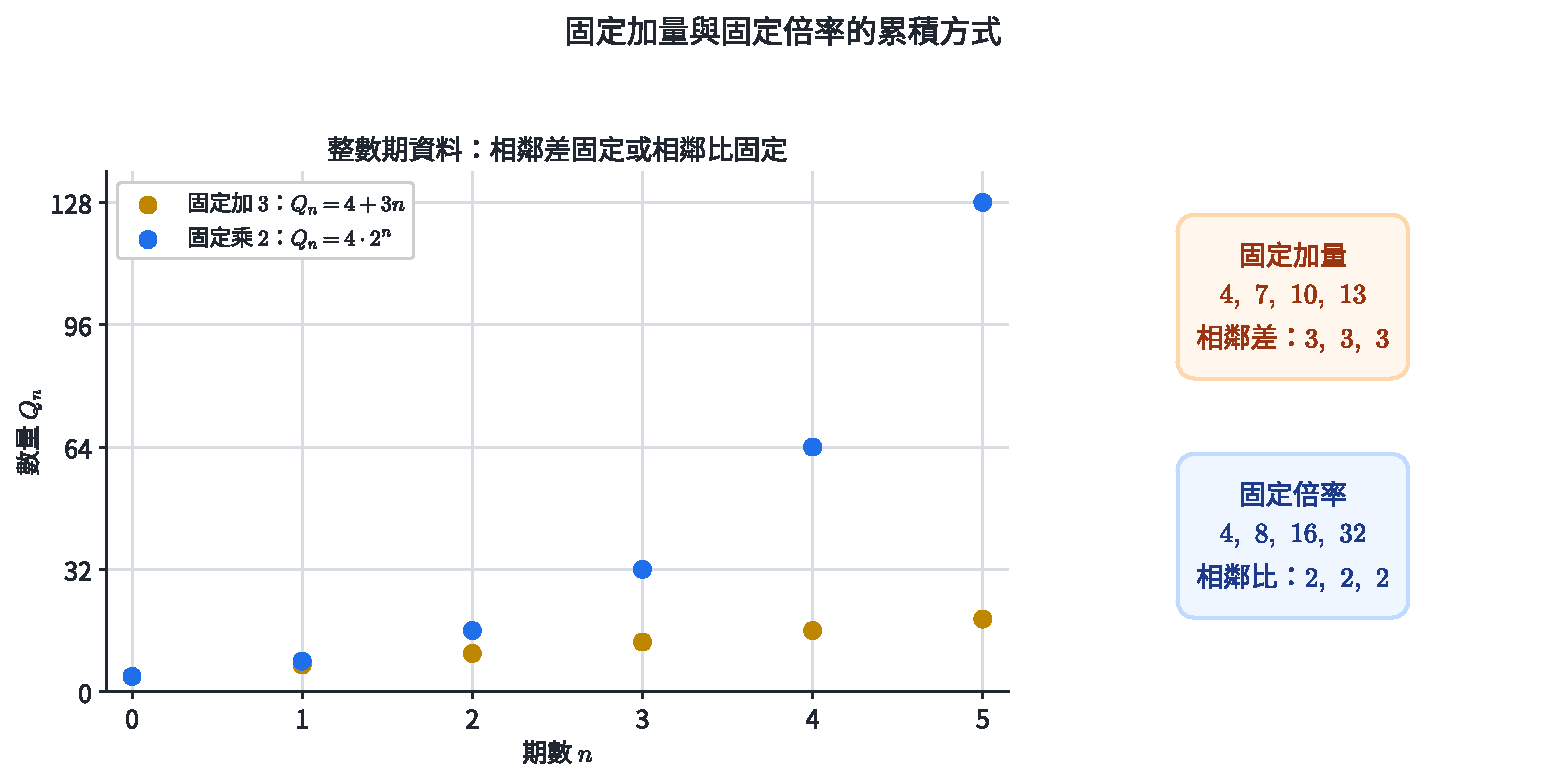
\includegraphics[width=0.94\linewidth,height=\textheight,keepaspectratio,alt={圖 2｜固定加量與固定倍率會產生不同的長期行為。}]{assets/數A3-2-線性與指數模型.pdf}
\caption{圖 2｜固定加量與固定倍率會產生不同的長期行為。}
\end{figure}

判斷模型時，應檢查相鄰等長時間區間的比值是否近似固定。真實資料含誤差時，倍率只會近似相同。

\begin{HandoutWorkedExample}

\subsection{完整示範｜把固定週期衰減寫進指數}\label{ux5b8cux6574ux793aux7bc4ux628aux56faux5b9aux9031ux671fux8870ux6e1bux5bebux9032ux6307ux6578}

某量起初為 \(800\)，每 \(3\) 小時剩原來的 \(3/4\)。令 \(t\) 以小時計：

\[
\boxed{Q(t)=800\left(\frac34\right)^{t/3}}.
\]

經過 \(9\) 小時是三個週期：

\[
Q(9)=800\left(\frac34\right)^3
=800\cdot\frac{27}{64}
=\boxed{337.5}.
\]

指數 \(t/3\) 的意義是「經過了幾個 3 小時」。

\end{HandoutWorkedExample}

\begin{HandoutWorkedExample}

\subsection{完整示範｜由資料的倍率建立模型}\label{ux5b8cux6574ux793aux7bc4ux7531ux8cc7ux6599ux7684ux500dux7387ux5efaux7acbux6a21ux578b}

某培養量的觀測值如下：

{\def\LTcaptype{none} % do not increment counter
\begin{longtable}[]{@{}rrrrr@{}}
\toprule\noalign{}
\(t\)（小時） & \(0\) & \(1\) & \(2\) & \(3\) \\
\midrule\noalign{}
\endhead
\bottomrule\noalign{}
\endlastfoot
\(Q(t)\) & \(120\) & \(150\) & \(187.5\) & \(234.375\) \\
\end{longtable}
}

相鄰比值都是

\[
\frac{150}{120}
=\frac{187.5}{150}
=\frac{234.375}{187.5}
=1.25.
\]

因此在這段資料所支持的範圍內，可用

\[
\boxed{Q(t)=120(1.25)^t}
\]

描述。預測 \(t=5\)：

\[
Q(5)=120(1.25)^5\approx\boxed{366.2}.
\]

資料只驗證前三個相鄰時段；若環境容量或資源限制開始影響倍率，後續需改用其他模型。

\end{HandoutWorkedExample}

\subsection{3.2 單利、複利與模型邊界}\label{ux55aeux5229ux8907ux5229ux8207ux6a21ux578bux908aux754c}

本金 \(P\)、每期利率 \(r\)、共 \(n\) 期：

\[
\boxed{\text{單利： }P(1+nr)},
\qquad
\boxed{\text{複利： }P(1+r)^n}.
\]

單利每期只按原本金計息，所以是固定增加；複利把已產生的利息併入下一期本金，所以是固定倍率。

\subsection{同樣寫「2\%」，單利與複利為何不同？}\label{ux540cux6a23ux5beb2ux55aeux5229ux8207ux8907ux5229ux70baux4f55ux4e0dux540c}

百分率只是每期的規則。單利的基準始終是原本金；複利的基準會隨本利和改變。公式前應先確認計息週期、利率是否為每期、是否有手續費與稅；課堂模型不等於真實商品報酬保證。

\begin{HandoutWorkedExample}

\subsection{完整示範｜複利達標時間用對數倒查}\label{ux5b8cux6574ux793aux7bc4ux8907ux5229ux9054ux6a19ux6642ux9593ux7528ux5c0dux6578ux5012ux67e5}

本金 \(80000\) 元，每年利率 \(3\%\)，每年複利一次。若條件維持，至少幾年後本利和達到 \(100000\) 元？

第 \(n\) 年末的本利和為

\[
A_n=80000(1.03)^n.
\]

要求 \(A_n\ge100000\)：

\[
(1.03)^n\ge1.25.
\]

底數 \(1.03>1\)，取對數後

\[
n\ge\frac{\log1.25}{\log1.03}\approx7.55.
\]

\(n\) 是完整計息期數，所以最小整數為 \(8\)：

\[
\boxed{8\text{ 年}}.
\]

檢查相鄰整數年：\(80000(1.03)^7\approx98390<100000\)，\(80000(1.03)^8\approx101341>100000\)。

\end{HandoutWorkedExample}

\subsection{3.3 對數尺度與演算法步數}\label{ux5c0dux6578ux5c3aux5ea6ux8207ux6f14ux7b97ux6cd5ux6b65ux6578}

對數適合描述跨越許多倍率的量。以分貝為例，若題目定義

\[
L=10\log\frac{I}{I_0},
\]

則強度比值相乘，分貝差會相加；強度變成 \(10\) 倍，聲音強度級增加 \(10\) dB。

\begin{figure}
\centering
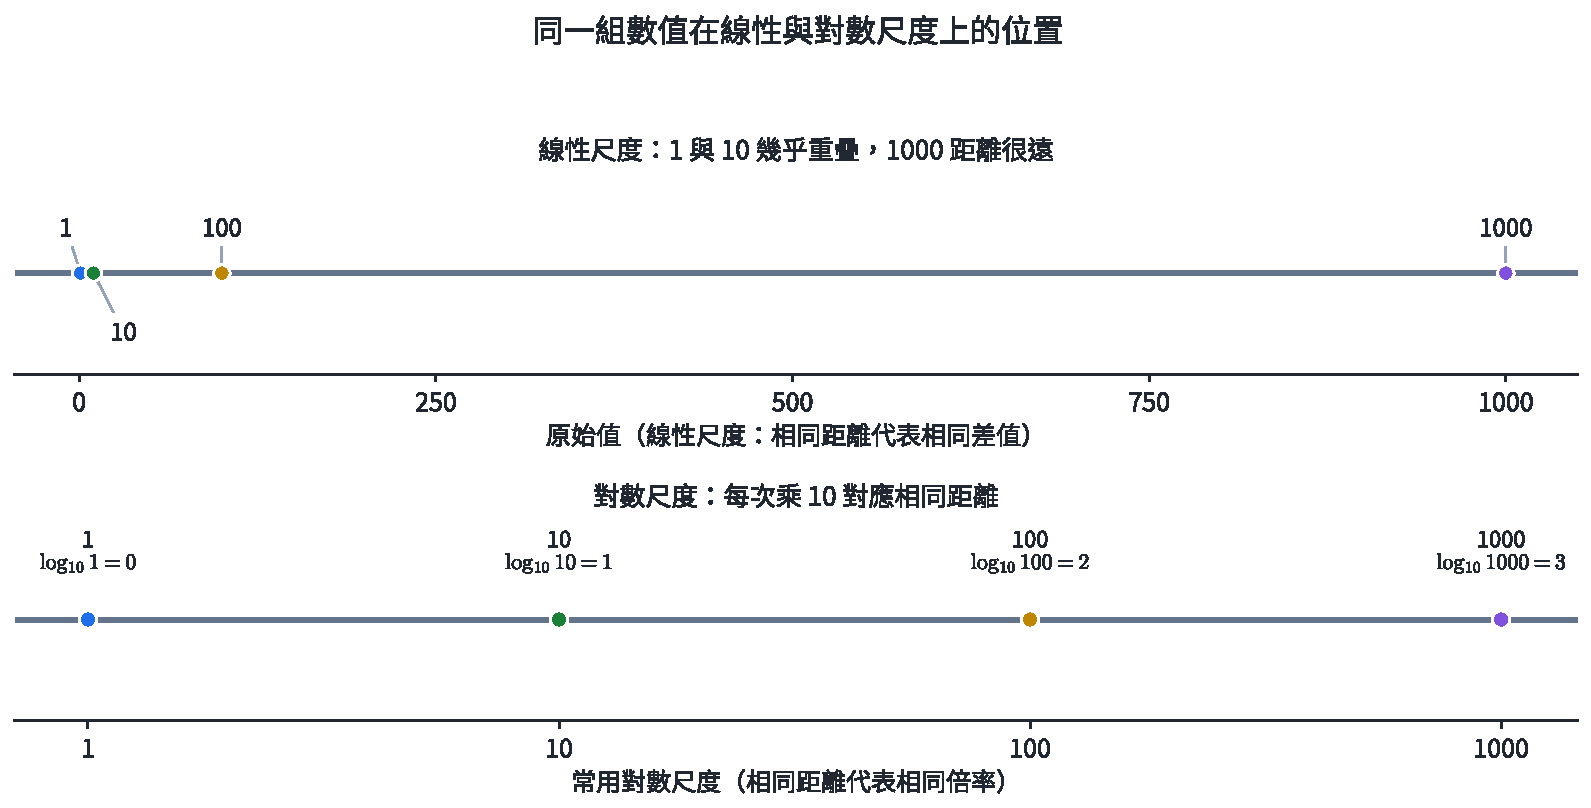
\includegraphics[width=0.92\linewidth,height=\textheight,keepaspectratio,alt={圖 3｜對數把每次乘 10 的區間壓成等距刻度。}]{assets/數A3-2-對數尺度.pdf}
\caption{圖 3｜對數把每次乘 10 的區間壓成等距刻度。}
\end{figure}

另一個真實用途是二分搜尋：每比較一次就把候選範圍約減半。若原有 \(N\) 筆資料，做 \(k\) 次後約剩 \(N/2^k\) 筆；要剩到 \(1\) 筆，需

\[
2^k\ge N
\quad\Longrightarrow\quad
k\ge\log_2N.
\]

例如 \(N=1024=2^{10}\)，最多約切 \(10\) 次。這個估計描述核心比較步數的數量級；實際總操作數還包含資料存取與其他程序。

\begin{HandoutWorkedExample}

\subsection{完整示範｜分貝差直接還原強度比}\label{ux5b8cux6574ux793aux7bc4ux5206ux8c9dux5deeux76f4ux63a5ux9084ux539fux5f37ux5ea6ux6bd4}

兩個聲音的強度級相差 \(18\) dB。由

\[
L_1-L_2=10\log\frac{I_1}{I_2}
\]

得到

\[
18=10\log\frac{I_1}{I_2}.
\]

所以

\[
\log\frac{I_1}{I_2}=1.8
\Longrightarrow
\boxed{\frac{I_1}{I_2}=10^{1.8}\approx63.1}.
\]

分貝差是對數差，還原後是強度的倍率；\(18\) dB 對應的強度比約為 \(63.1\)。

\end{HandoutWorkedExample}

\subsection{對數尺度如何壓縮大範圍？}\label{ux5c0dux6578ux5c3aux5ea6ux5982ux4f55ux58d3ux7e2eux5927ux7bc4ux570d}

\textbf{倍率造成的跨度。} \(1,10,100,1000\) 每次乘 \(10\)，差距愈來愈大。

\textbf{對數把倍率轉成等距。} \(\log1,\log10,\log100,\log1000\) 變成 \(0,1,2,3\)，每個倍率十倍都只往前一格。

\textbf{讀圖用途與限制。} 圖表能同時容納很小與很大的量，且相同距離代表相同倍數。讀圖時須確認座標軸尺度；對數尺度的一格表示固定倍率。

\begin{HandoutSelfCheck}

\subsection{節末練習｜成長、衰退、複利與尺度}\label{ux7bc0ux672bux7df4ux7fd2ux6210ux9577ux8870ux9000ux8907ux5229ux8207ux5c3aux5ea6}

\begin{enumerate}
\def\labelenumi{\arabic{enumi}.}
\tightlist
\item
  某量每 \(4\) 小時變為原來的 \(80\%\)。若初值為 \(500\)，寫出 \(Q(t)\)，並求 \(t=12\) 的值。
\item
  資料 \(40,52,67.6,87.88\) 是線性或指數型？寫出以首項為 \(Q(0)\) 的模型。
\item
  本金 \(50000\) 元，年利率 \(4\%\)，每年複利一次。三年後本利和為何？
\item
  某量依 \(Q(t)=900(0.7)^t\) 變化。求首次低於 \(200\) 的最小整數 \(t\)。
\item
  強度變為原來的 \(1000\) 倍時，依 \(L=10\log(I/I_0)\)，強度級增加多少 dB？
\item
  二分搜尋處理 \(5000\) 筆已排序資料，若每次把候選數量至多減半，至少需取哪個整數 \(k\) 才保證 \(2^k\ge5000\)？
\end{enumerate}

\textbf{答案：}

\begin{enumerate}
\def\labelenumi{\arabic{enumi}.}
\tightlist
\item
  \(Q(t)=500(0.8)^{t/4}\)；\(Q(12)=500(0.8)^3=256\)。
\item
  相鄰倍率皆為 \(1.3\)，是指數型；\(Q(n)=40(1.3)^n\)。
\item
  \(50000(1.04)^3=56243.2\) 元。
\item
  \(t>\log(200/900)/\log0.7\approx4.22\)，最小整數為 \(5\)。
\item
  \(10\log1000=30\) dB。
\item
  \(2^{12}=4096<5000<8192=2^{13}\)，所以 \(k=13\)。
\end{enumerate}

\end{HandoutSelfCheck}

\section{4. 一頁核心整理}\label{ux4e00ux9801ux6838ux5fc3ux6574ux7406}

\subsection{指數}\label{ux6307ux6578}

\begin{itemize}
\tightlist
\item
  \(a^x\)：\(a>0\)、\(a\ne1\)；定義域 \(\mathbb R\)，值域 \((0,\infty)\)。
\item
  \(a>1\) 遞增；\(0<a<1\) 遞減。
\item
  固定倍率模型：\(Q(t)=Q_0a^t\)。
\item
  不等式去掉底數時，方向由單調性決定。
\item
  \(a^{2x}\)、\(a^x\) 同時出現時可令 \(t=a^x>0\)；異底方程可取對數。
\end{itemize}

\subsection{對數}\label{ux5c0dux6578}

\begin{itemize}
\tightlist
\item
  \(\log_ax=y\iff a^y=x\)；真數 \(x>0\)。
\item
  對數與指數互為反函數，圖形對 \(y=x\) 對稱。
\item
  平移後先由真數條件找定義域與鉛直漸近線，再判單調性與截距。
\item
  積變和、商變差、冪變乘法；真數的加減結構須原樣保留。
\item
  換底：\(\log_ab=\log b/\log a\)。
\item
  \(\ln x=\log_e x\)；\(e\approx2.718\) 可由複利切分的極限動機理解。
\item
  解方程與不等式時，先列真數條件，最後再驗。
\end{itemize}

\subsection{使用模型前}\label{ux4f7fux7528ux6a21ux578bux524d}

\begin{itemize}
\tightlist
\item
  固定增加看差；固定倍率看比。
\item
  複利、衰減模型須對齊計息或變化週期。
\item
  對數尺度的一格代表固定倍率；線性尺度的一格才代表固定差值。
\end{itemize}

\section{5. 分層題與跨節整合題}\label{ux5206ux5c64ux984cux8207ux8de8ux7bc0ux6574ux5408ux984c}

\subsection{題目 1｜圖形性質}\label{ux984cux76ee-1ux5716ux5f62ux6027ux8cea}

對

\[
f(x)=\left(\frac13\right)^{x-2}+1,
\]

求定義域、值域、單調性、水平漸近線與 \(f(2)\)。

\subsection{題目 2｜指數方程式}\label{ux984cux76ee-2ux6307ux6578ux65b9ux7a0bux5f0f}

解

\[
9^x-10\cdot3^x+9=0.
\]

\subsection{題目 3｜指數不等式}\label{ux984cux76ee-3ux6307ux6578ux4e0dux7b49ux5f0f}

解

\[
\left(\frac14\right)^{x+1}<8^{\,1-2x}.
\]

\subsection{題目 4｜對數律與換底}\label{ux984cux76ee-4ux5c0dux6578ux5f8bux8207ux63dbux5e95}

已知 \(\log2\approx0.3010\)、\(\log3\approx0.4771\)：

\begin{enumerate}
\def\labelenumi{\arabic{enumi}.}
\tightlist
\item
  估算 \(\log24\)；
\item
  將 \(\log_2 7\) 寫成常用對數的比值。
\end{enumerate}

\subsection{題目 5｜對數方程式}\label{ux984cux76ee-5ux5c0dux6578ux65b9ux7a0bux5f0f}

解

\[
\log_3(x-1)+\log_3(x-3)=2.
\]

\subsection{題目 6｜對數不等式}\label{ux984cux76ee-6ux5c0dux6578ux4e0dux7b49ux5f0f}

解

\[
\log_{1/3}(2x-1)\le-1.
\]

\subsection{題目 7｜複利與達標時間}\label{ux984cux76ee-7ux8907ux5229ux8207ux9054ux6a19ux6642ux9593}

本金 \(100000\) 元，以每年 \(2\%\)、每年複利一次計息：

\begin{enumerate}
\def\labelenumi{\arabic{enumi}.}
\tightlist
\item
  五年後本利和約多少元？
\item
  若利率與規則維持不變，至少幾年後本利和超過 \(120000\) 元？可用計算機。
\end{enumerate}

\subsection{題目 8｜分貝是倍率問題}\label{ux984cux76ee-8ux5206ux8c9dux662fux500dux7387ux554fux984c}

聲音強度級定義為

\[
L=10\log\frac{I}{I_0}\quad(\mathrm{dB}).
\]

\begin{enumerate}
\def\labelenumi{\arabic{enumi}.}
\tightlist
\item
  甲、乙兩處分別為 \(70\) dB、\(40\) dB，甲的聲音強度是乙的幾倍？
\item
  若強度變為原來的兩倍，聲音強度級增加多少 dB？取 \(\log2\approx0.3010\)。
\end{enumerate}

\subsection{題目 9｜對數圖形變換}\label{ux984cux76ee-9ux5c0dux6578ux5716ux5f62ux8b8aux63db}

對

\[
g(x)=-\log_2(x+1)+3,
\]

求定義域、值域、鉛直漸近線、單調性與 \(x\) 截距。

\subsection{題目 10｜異底指數方程式}\label{ux984cux76ee-10ux7570ux5e95ux6307ux6578ux65b9ux7a0bux5f0f}

解

\[
2^{x+1}=7^x,
\]

並給出到小數第二位的近似值。

\subsection{題目 11｜異底對數不等式}\label{ux984cux76ee-11ux7570ux5e95ux5c0dux6578ux4e0dux7b49ux5f0f}

解

\[
\log_3x\le\log_9(3x).
\]

\subsection{題目 12｜指數代換與極值}\label{ux984cux76ee-12ux6307ux6578ux4ee3ux63dbux8207ux6975ux503c}

求

\[
f(x)=4^x-10\cdot2^x+9
\]

的最小值與取得位置。

\subsection{題目 13｜跨節整合：由資料判定模型並反求時間}\label{ux984cux76ee-13ux8de8ux7bc0ux6574ux5408ux7531ux8cc7ux6599ux5224ux5b9aux6a21ux578bux4e26ux53cdux6c42ux6642ux9593}

某量的紀錄如下：

{\def\LTcaptype{none} % do not increment counter
\begin{longtable}[]{@{}rrrr@{}}
\toprule\noalign{}
\(t\) & \(0\) & \(2\) & \(4\) \\
\midrule\noalign{}
\endhead
\bottomrule\noalign{}
\endlastfoot
\(Q(t)\) & \(200\) & \(288\) & \(414.72\) \\
\end{longtable}
}

\begin{enumerate}
\def\labelenumi{\arabic{enumi}.}
\tightlist
\item
  檢查每兩個時間單位的倍率，建立指數模型；
\item
  依此模型，何時首次達到 \(600\)？答案取到小數第二位。
\end{enumerate}

\subsection{題目 14｜跨節整合：圖形交點的個數與位置}\label{ux984cux76ee-14ux8de8ux7bc0ux6574ux5408ux5716ux5f62ux4ea4ux9edeux7684ux500bux6578ux8207ux4f4dux7f6e}

考慮

\[
2^x=4-x.
\]

\begin{enumerate}
\def\labelenumi{\arabic{enumi}.}
\tightlist
\item
  說明此方程至多有一個實根；
\item
  用 \(x=1,1.5,2\) 的函數值夾出根所在區間；
\item
  用計算機求根到小數第二位。
\end{enumerate}

\subsection{題目 15｜跨節整合：每月複利與達標期數}\label{ux984cux76ee-15ux8de8ux7bc0ux6574ux5408ux6bcfux6708ux8907ux5229ux8207ux9054ux6a19ux671fux6578}

本金 \(120000\) 元，名目年利率 \(4.8\%\)，每月利率按 \(0.048/12\) 計，每月底複利一次。

\begin{enumerate}
\def\labelenumi{\arabic{enumi}.}
\tightlist
\item
  寫出 \(n\) 個月後本利和；
\item
  至少幾個月後超過 \(130000\) 元？
\end{enumerate}

\subsection{題目 16｜跨節整合：資料量與搜尋步數}\label{ux984cux76ee-16ux8de8ux7bc0ux6574ux5408ux8cc7ux6599ux91cfux8207ux641cux5c0bux6b65ux6578}

一份已排序資料每年成長為前一年的 \(1.5\) 倍，目前有 \(20000\) 筆。

\begin{enumerate}
\def\labelenumi{\arabic{enumi}.}
\tightlist
\item
  建立 \(t\) 年後的資料量模型；
\item
  求首次超過 \(100000\) 筆的最小整數年數；
\item
  到那一年，二分搜尋至少取哪個整數 \(k\) 才有 \(2^k\) 不小於資料筆數？
\end{enumerate}

\clearpage

\section{6. 分層題與跨節整合題詳解}\label{ux5206ux5c64ux984cux8207ux8de8ux7bc0ux6574ux5408ux984cux8a73ux89e3}

\subsection{第 1 題}\label{ux7b2c-1-ux984c}

底數 \(1/3\) 介於 \(0\) 與 \(1\) 之間，所以函數嚴格遞減。基本函數值域 \((0,\infty)\)，再向上平移 \(1\)：

\[
\boxed{\text{定義域 }\mathbb R,\quad
\text{值域 }(1,\infty)}.
\]

水平漸近線為 \(\boxed{y=1}\)。代入 \(x=2\)：

\[
f(2)=\left(\frac13\right)^0+1=\boxed2.
\]

\subsection{第 2 題}\label{ux7b2c-2-ux984c}

令 \(t=3^x>0\)，則 \(9^x=t^2\)：

\[
t^2-10t+9=(t-1)(t-9)=0.
\]

所以 \(t=1\) 或 \(9\)。回代：

\[
3^x=1\Rightarrow x=0,\qquad
3^x=9\Rightarrow x=2.
\]

故 \(\boxed{x=0,2}\)。

\subsection{第 3 題}\label{ux7b2c-3-ux984c}

全部化為底數 \(2\)：

\[
\left(\frac14\right)^{x+1}
=2^{-2x-2},
\qquad
8^{1-2x}=2^{3-6x}.
\]

因底數 \(2>1\)，比較指數時方向不變：

\[
-2x-2<3-6x
\Rightarrow4x<5
\Rightarrow\boxed{x<\frac54}.
\]

\subsection{第 4 題}\label{ux7b2c-4-ux984c}

因 \(24=2^3\cdot3\)，

\[
\log24=3\log2+\log3
\approx3(0.3010)+0.4771
=\boxed{1.3801}.
\]

換底公式給出

\[
\boxed{\log_2 7=\frac{\log7}{\log2}}.
\]

\subsection{第 5 題}\label{ux7b2c-5-ux984c}

先列真數條件：

\[
x-1>0,\quad x-3>0
\Rightarrow x>3.
\]

合併對數：

\[
\log_3[(x-1)(x-3)]=2
\Rightarrow(x-1)(x-3)=9.
\]

\[
x^2-4x-6=0
\Rightarrow
x=2\pm\sqrt{10}.
\]

因 \(2-\sqrt{10}<3\)，捨去；所以

\[
\boxed{x=2+\sqrt{10}}.
\]

\subsection{第 6 題}\label{ux7b2c-6-ux984c}

先有 \(2x-1>0\)，即 \(x>1/2\)。因底數 \(1/3<1\)，函數遞減：

\[
\log_{1/3}(2x-1)\le-1
\iff
2x-1\ge(1/3)^{-1}=3.
\]

所以 \(2x\ge4\)，得

\[
\boxed{x\ge2}.
\]

這已自動滿足真數條件。

\subsection{第 7 題}\label{ux7b2c-7-ux984c}

五年後本利和為

\[
100000(1.02)^5
\approx100000(1.1040808)
\approx\boxed{110408\text{ 元}}.
\]

要超過 \(120000\)：

\[
100000(1.02)^n>120000
\iff
(1.02)^n>1.2.
\]

取對數：

\[
n>\frac{\log1.2}{\log1.02}
\approx9.21.
\]

\(n\) 是完整計息年數，所以至少要 \(\boxed{10\text{ 年}}\)。檢查：\((1.02)^9\approx1.1951<1.2\)，\((1.02)^{10}\approx1.2190>1.2\)。

\subsection{第 8 題}\label{ux7b2c-8-ux984c}

兩地的分貝差為

\[
70-40
=10\log\frac{I_{\text{甲}}}{I_{\text{乙}}}
=30.
\]

因此

\[
\log\frac{I_{\text{甲}}}{I_{\text{乙}}}=3
\Rightarrow
\boxed{\frac{I_{\text{甲}}}{I_{\text{乙}}}=10^3=1000}.
\]

若強度變兩倍，增加量為

\[
\Delta L
=10\log\frac{2I}{I}
=10\log2
\approx\boxed{3.01\ \mathrm{dB}}.
\]

分貝差對應強度倍率；強度合成需先回到強度尺度處理。

\subsection{第 9 題}\label{ux7b2c-9-ux984c}

真數條件 \(x+1>0\) 給出定義域

\[
\boxed{x>-1}.
\]

當 \(x\to-1^+\) 時，真數趨近 \(0^+\)，所以鉛直漸近線是 \(\boxed{x=-1}\)。基本函數 \(\log_2(x+1)\) 遞增，外面的負號使 \(g\) 嚴格遞減；鉛直平移不改變值域，因此值域為 \(\mathbb R\)。

\(x\) 截距滿足

\[
-\log_2(x+1)+3=0
\Longrightarrow
\log_2(x+1)=3.
\]

所以 \(x+1=8\)，即截距為

\[
\boxed{(7,0)}.
\]

\subsection{第 10 題}\label{ux7b2c-10-ux984c}

兩邊取自然對數：

\[
(x+1)\ln2=x\ln7.
\]

整理得

\[
x(\ln7-\ln2)=\ln2,
\]

所以

\[
\boxed{x=\frac{\ln2}{\ln7-\ln2}}
\approx\boxed{0.55}.
\]

\subsection{第 11 題}\label{ux7b2c-11-ux984c}

真數條件為 \(x>0\)。把右邊換成以 \(3\) 為底：

\[
\log_9(3x)
=\frac{\log_3(3x)}{\log_39}
=\frac12(1+\log_3x).
\]

所以

\[
\log_3x\le\frac12(1+\log_3x)
\Longrightarrow
\log_3x\le1.
\]

底數 \(3>1\)，故 \(x\le3\)。與定義域取交集：

\[
\boxed{0<x\le3}.
\]

\subsection{第 12 題}\label{ux7b2c-12-ux984c}

令 \(t=2^x>0\)，則

\[
f=t^2-10t+9=(t-5)^2-16.
\]

\(t=5\) 符合 \(t>0\)，所以最小值為

\[
\boxed{-16}.
\]

由 \(2^x=5\) 得取得位置

\[
\boxed{x=\log_2 5}.
\]

\subsection{第 13 題}\label{ux7b2c-13-ux984c}

每兩個時間單位的倍率為

\[
\frac{288}{200}=1.44,
\qquad
\frac{414.72}{288}=1.44.
\]

因此

\[
Q(t)=200(1.44)^{t/2}.
\]

因 \(1.44=(1.2)^2\)，也可寫成

\[
\boxed{Q(t)=200(1.2)^t}.
\]

求 \(Q(t)=600\)：

\[
200(1.2)^t=600
\Longrightarrow
(1.2)^t=3.
\]

所以

\[
t=\frac{\log3}{\log1.2}
\approx\boxed{6.03}.
\]

\subsection{第 14 題}\label{ux7b2c-14-ux984c}

\(y=2^x\) 嚴格遞增，\(y=4-x\) 嚴格遞減，所以兩圖至多相交一次。

比較三個位置：

{\def\LTcaptype{none} % do not increment counter
\begin{longtable}[]{@{}rrrl@{}}
\toprule\noalign{}
\(x\) & \(2^x\) & \(4-x\) & 比較 \\
\midrule\noalign{}
\endhead
\bottomrule\noalign{}
\endlastfoot
\(1\) & \(2\) & \(3\) & 左邊較小 \\
\(1.5\) & 約 \(2.828\) & \(2.5\) & 左邊較大 \\
\(2\) & \(4\) & \(2\) & 左邊較大 \\
\end{longtable}
}

因此根在 \((1,1.5)\)。用計算機求得

\[
\boxed{x\approx1.39}.
\]

單調性保證這個近似值對應唯一實根。

\subsection{第 15 題}\label{ux7b2c-15-ux984c}

每月利率為

\[
\frac{0.048}{12}=0.004.
\]

\(n\) 個月後本利和為

\[
\boxed{A_n=120000(1.004)^n}.
\]

要求 \(A_n>130000\)：

\[
(1.004)^n>\frac{13}{12}.
\]

取對數：

\[
n>\frac{\log(13/12)}{\log1.004}
\approx20.05.
\]

最小整數為 \(\boxed{21}\)。檢查：第 \(20\) 個月約為 \(129974\) 元，第 \(21\) 個月約為 \(130494\) 元。

\subsection{第 16 題}\label{ux7b2c-16-ux984c}

\(t\) 年後的資料量為

\[
\boxed{N(t)=20000(1.5)^t}.
\]

要超過 \(100000\)：

\[
(1.5)^t>5
\Longrightarrow
t>\frac{\log5}{\log1.5}
\approx3.97.
\]

最小整數年數為 \(\boxed{4}\)，屆時

\[
N(4)=20000(1.5)^4=101250.
\]

又

\[
2^{16}=65536<101250<131072=2^{17},
\]

所以需取 \(\boxed{k=17}\)。


\end{document}
